\chapter{Theoretische Grundlagen}
Dieses Kapitel eruiert die theoretischen Grundlagen für die Ausarbeitung, welche für das Verständnis dieser Arbeit notwendig sind und im praktischen Teil angewendet werden.
\section{WordPress als Content-Management-System}
WordPress ist ein freies, unter der \gls{gnu} \gls{gpl} v2 lizenziertes Content-Management-System und mit einem Marktanteil von 61,1\% das weltweit am häufigsten verwendete CMS. \cite{statista2025cms}
Die Plattform zeichnet sich durch seine flexibilität, erweiterbarkeit und bedienbarkeit aus, was Wordpress zu einer Lösung für simple Webseiten und Blogs bis hin zu komplexe Web-Applikationen. \cite{patel2019review}
Die technische Struktur verfolgt ein modulares Paradigma, das eine klare Trennung zwischen Kernfunktionen, Design und Erweiterungen ermöglicht:
\begin{itemize}

 \item Themes: Kontrollieren die Präsentationslogik und das Design der Webseite

 \item Plugins: Erweitern die Funktionalität

 \item Core System: Stellt die grundlegenden Funktionen des CMS bereit

\end{itemize}
Technisch gesehen besteht Wordpress aus einer \gls{php}-basierten Architektur in Verbindung mit der persistenten Speicherlösung \gls{mysql} als relationale Datenbank.
Durch diese weit verbreiteten Technologien ist WordPress mit den meisten gängigen Hosting-Umgebungen kompatibel.
Grundlage hierfür ist lediglich ein Webserver, welcher PHP und MySQL unterstützt.
Offiziell ist Apache oder Nginx empfohlen \cite{wordpress2024requirements}.

Darüber hinaus bietet Wordpress eine \gls{rest}-\gls{api} mit der eine entkoppelte Inhaltsverwaltung möglich ist und Inhalte über das \gls{http}-Protokoll in verschiedene Anwendungen und Plattformen integriert werden können.
\newpage
\textbf{WordPress Coding Standards und Code-Qualität}\\
Wordpress Coding Standards dienen als Richtlinien und Best Practises für Entwickler die an Wordpress Projekten arbeiten.
Diese Standards haben sich in der Wordpress Community etabliert und ermöglichen eine konsistente Codestruktur.
Hintergrund ist es die Codebasis für bessere Wartbarkeit und kollaborative Arbeit zu strukturieren.
Für die Ausarbeitung der Weiterentwicklung sollen die offiziellen Wordpress Coding Standards beachtet und umgesetzt werden.


\section{Plugin-Entwicklung mit WordPress}

Die offizielle WordPress-Definition besagt: \glqq Plugins sind Codepakete, die die Kernfunktionalität von WordPress erweitern.
WordPress-Plugins bestehen aus PHP-Code und können weitere Assets wie Bilder,
CSS und JavaScript enthalten\grqq{} \cite{wordpress2024plugin} (eigene Übersetzung).
\\
Für die Entwicklung solcher Plugins ist grundlegend ein tiefergehendes Verständnis des Wordpress-CMS vorausgesetzt.
Die Grundlagen sowie weiterführende Themengebiete sollen im Folgenden ermittelt werden.



\subsection{Grundlagen der Plugin-Architektur}

Die Entwicklung von Plugins in WordPress setzt ein grundlegendes Verständnis der Dateistruktur und des internen Aufbaus des Content-Management-Systems voraus.
Insbesondere ist es erforderlich, die Plugin-bezogenen Dateien korrekt zu strukturieren und im entsprechenden Verzeichnis innerhalb der WordPress-Installation zu platzieren.\\\\
Plugins werden standardmäßig im Verzeichnis wp-content/plugins abgelegt.
Jeder Plugin-Ordner enthält dabei alle notwendigen Dateien zur Funktionalität des jeweiligen Moduls.\\\\
Im folgenden Schaubild ist eine typische, nicht modifizierte Verzeichnisstruktur einer WordPress-Installation dargestellt.
Diese dient als Ausgangspunkt für die Entwicklung und Integration von Plugins:

\begin{figure}[tbh]
 \centering
 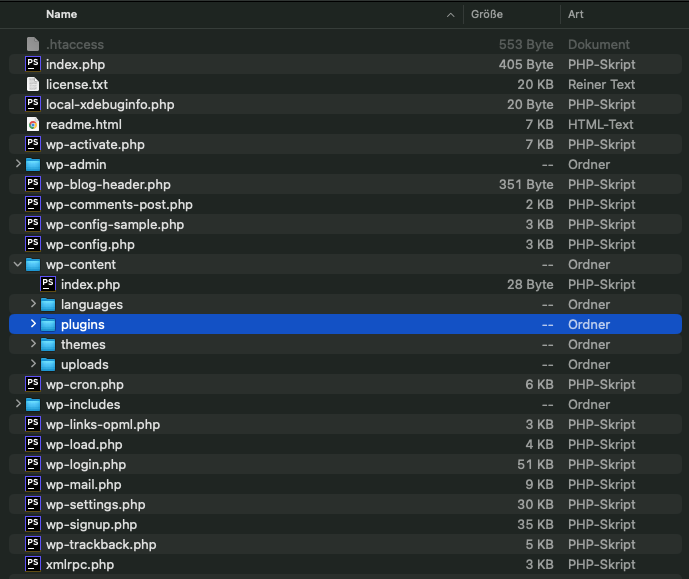
\includegraphics[width=0.88\textwidth]{wordpress_ordner_aufbau}
 \caption{Unveränderte WordPress-Verzeichnisstruktur (6.8.2)}
 \label{fig:wordpress-verzeichnis}
\end{figure}
\newpage
Abbildung 2.1 visualisiert, dass sich im wp-content Ordner bereits initial in der Standardkonfiguration von Wordpress das Verzeichnis plugins befindet.
Der plugins Ordner ist die zentrale Destination für alle im Wordpress System erstellten Erweiterungen.
Die nachfolgende Untersuchung berücksichtigt weitere Bestandteile von WordPress-Plugins, die fortlaufend detailliert beschrieben werden.
\\\\\\
\textbf{Aufbau, Plugin-Header und Metadateien}

Für die Entwicklung von WordPress-Plugins empfehlen die offiziellen WordPress Developer Resources eine klare und strukturierte Ordnerorganisation\cite{wordpress2024BestPractices}.
Als Empfohlen wird folgende grundlegende Verzeichnisstruktur vorgeschlagen:
\\\\\\
\begin{lstlisting}[caption={Beispielhafte Plugin-Verzeichnisstruktur in WordPress}, label={lst:plugin-structure}]
/plugin-name
│
├── plugin-name.php
├── uninstall.php
│
├── /languages
├── /includes
│
├── /admin
│   ├── /js
│   ├── /css
│   └── /images
│
└── /public
    ├── /js
    ├── /css
    └── /images
\end{lstlisting}

Die plugin-name.php gibt im oben gezeigten Beispielaufbau die zentrale Plugindatei an.
Diese Datei muss damit der Ordner als Plugin verstanden wird einen von Wordpress vorgegebene Headerstrutkur enthalten.
Das Minimum des Header ist wie folgt definiert:

\begin{lstlisting}[caption={Minimaler Plugin-Header in WordPress}, label={lst:plugin-header}]
<?php
/*
 * Plugin Name: YOUR PLUGIN NAME
 */
\end{lstlisting}

Darüber hinaus können weitere optionale Felder definiert werden wie:
\texttt{Author URI} für die Website des Plugin-Entwicklers, \texttt{Text Domain}
zur Internationalisierung und \texttt{Domain Path} für den Pfad zu Sprachdateien.
Alle möglichen Felder werden in der folgenden Tabelle aufgeführt:
\renewcommand{\arraystretch}{1.3}

\begin{longtable}{>{\bfseries}p{4cm} p{10cm}}
 \caption{Übersicht der Plugin-Header-Felder in WordPress} \\
 \hline
 Feldname & Beschreibung \\
 \hline
 \endfirsthead

 \multicolumn{2}{l}{\textit{Fortsetzung von vorheriger Seite}} \\
 \hline
 Feldname & Beschreibung \\
 \hline
 \endhead

 \hline
 \multicolumn{2}{r}{\textit{Fortsetzung auf nächster Seite}} \\
 \endfoot

 \hline
 \endlastfoot

 Plugin Name (erforderlich) & Der Name des Plugins, wie er in der Plugin-Übersicht im WordPress-Adminbereich angezeigt wird. \\
 Plugin URI & Eine eindeutige URL zur Startseite des Plugins, idealerweise auf der eigenen Website. WordPress.org-URLs sind hier nicht erlaubt. \\
 Description & Eine kurze Beschreibung des Plugins (max. 140 Zeichen), wie sie im WordPress-Adminbereich angezeigt wird. \\
 Version & Die aktuelle Versionsnummer des Plugins, z.\,B. \texttt{1.0} oder \texttt{1.0.3}. \\
 Requires at least & Die minimale WordPress-Version, mit der das Plugin kompatibel ist. \\
 Requires PHP & Die minimale benötigte PHP-Version für das Plugin. \\
 Author & Der Name des Autors oder der Autoren des Plugins. Mehrere Autoren können durch Kommas getrennt angegeben werden. \\
 Author URI & Die Website des Autors oder ein öffentliches Profil, z.\,B. auf WordPress.org. \\
 License & Die Kurzbezeichnung der Lizenz, unter der das Plugin veröffentlicht wird (z.\,B. \texttt{GPLv2}). \\
 License URI & Ein Link zum vollständigen Lizenztext (z.\,B. \url{https://www.gnu.org/licenses/gpl-2.0.html}). \\
 Text Domain & Die Textdomain für die Internationalisierung des Plugins, erforderlich für Übersetzungen mit \texttt{gettext}. \\
 Domain Path & Das Verzeichnis, in dem WordPress die Übersetzungsdateien findet (z.\,B. \texttt{/languages}). \\
 Network & Gibt an, ob das Plugin netzwerkweit (Multisite) aktiviert werden kann. Nur \texttt{true} ist erlaubt, andernfalls Feld weglassen. \\
 Update URI & Eine eindeutige URI zur Updatequelle, um versehentliche Überschreibungen durch gleichnamige Plugins im WordPress.org-Verzeichnis zu vermeiden. \\
 Requires Plugins & Eine durch Kommas getrennte Liste von Plugin-Slugs aus dem WordPress.org-Verzeichnis, die als Abhängigkeit benötigt werden. Kommas innerhalb der Slugs sind nicht erlaubt. \\
\end{longtable}

\newpage
\textbf{Hooks: Action und Filter}\\\\
Hooks erlauben es an spezifischen Stellen einzugreifen, um das Verhalten von Wordpress zu ändern ohne dabei die Kern-Dateien bearbeiten zu müssen.
Allgemein gibt es zwei Arten von hooks in Wordpress: Actions und Filter.
Mit Actions können Funktionen hinzugefügt oder geändert werden während Filter Inhalte geändert werden können, während diese geladen und dem Website-Nutzer angezeigt werden.
Hooks sind nicht nur für die Plugin-Entwicklung gedacht, sondern werden ebenfalls häufig verwendet, um Standardfunktionen durch den Wordpress-Kern selbst bereitzustellen.

Zu den drei wichtigsten Hooks im Bereich der Plugins zählen der register\_activation\_hook(), register\_deactivation\_hook() und der register\_uninstall\_hook().

\begin{itemize}
 \item register\_activation\_hook(): Dieser Hook wird ausgeführt, wenn das Plugin im Wordpress-Backend aktiviert wird. Dies wird oftmals verwendet um Funktionen zwecks Einrichtung des Plugins bereitzustellen.
 \item register\_deactivation\_hook(): Der Deaktivierung-Hook wird ausgeführt, wenn das Plugin deaktiviert wird. Diese Funktion ermöglicht es die vom Plugin temporär gespeicherten Daten und Einträge zu entfernen.
 \item register\_uninstall\_hook(): Die Ausführung hier findet statt, wenn das Plugin aus dem Backend gelöscht wird. Die Verwendung zielt häufig darauf ab alle vom Plugin erstellen Optionen oder Datenbanktabellen restlos zu löschen.
\end{itemize}

%Plugin-Struktur und -Organisation

%Das WordPress Hook-System verstehen

%Plugin-Header und Metadaten

%Aktivierung und Deaktivierung von Plugins

%Plugin-Hauptdatei und Ordnerstruktur

\textbf{Best Practises in der Plugin-Programmierung}\\\\
Das Plugin Handbuch von Wordpress gibt dem Entwickler einige Best Practises vor, welche helfen den Code zu organisieren.
Ferner wird durch die Hinweise sichergestellt, dass der Code gut mit dem Wordpress Kern und anderen Plugins funktioniert.
\\
\\
\texttt{Vermeiden von Namenskonflikten:}\\
Namenskollisionen können durch die gleiche Benennung von Variablen, Funktionen oder Klassen zustandekommen.
Um einen solchen Namenskonflikt zu vermeiden ist es empfohlen einen globalen Namenspace zu definieren. Dieser Namespace ermöglicht das überschreiben von anderen Variablen, Funktionen und Plugins.
Variablen die innerhalb von Funktionen oder Klassen definiert sind, sind hiervon nicht betroffen.
\\
\\
\texttt{Voranstellen eines Prefix}\\
Unter Zuhilfenahme eines Prefix können potenzielle Konflikte im Hinblick auf Aufrufe und Ausführungen mit anderen Plugins verhindert werden.
Das Handbuch empfiehlt hierzu ein 4 oder 5 zeichen langes einzigartiges Wort, welches vor verschiedene deklarationen vorangestellt wird.
Auf das Projekt ChariGame gemünzte Projekt könnte dies dann wie folgt aussehen:
\begin{itemize}

 \item function charigame\_save\_post();

 \item define ('CHARIGAME\_LICENSE', true);

 \item class CHARIGAME\_Admin{}

 \item namespace ChariGame;

 \item update\_option('charigame\_settings', $settings)
\end{itemize}

Auf vorhandene Implementierungen prüfen:






Internationalisierung (i18n)

\subsection{Schnittstellen und Interfaces}

Admin-Menüs und Unterseiten erstellen

Meta-Daten // Meta Boxes für Post-Bearbeitung

Einstellungsseiten mit Settings \gls{api}

Integration mit \gls{acf} für erweiterte Felder

Shortcodes entwickeln und registrieren

Custom Widgets erstellen

\gls{css} und JavaScript richtig einbinden

Gutenberg Block-Entwicklung (optional)

Custom \gls{rest} \gls{api} Endpoints erstellen

Daten über \gls{http}-Requests bereitstellen

Authentifizierung und Berechtigungen

AJAX-Funktionalität implementieren

\subsection{Plugin-Deployment und Distribution}

WordPress Database \gls{api} für Datenbankoperationen

Custom Post Types und Custom Fields

Settings und Options verwalten

Caching mit Transients

Plugin für WordPress Repository vorbereiten

Versionskontrolle und Updates

Lizenzierung unter \gls{gpl}

Plugin-Testing und Qualitätssicherung

\subsection{Performance und Sicherheit}

Sicherheitsaspekte (Sanitization, Validation, Nonces)

Performance-Optimierung

Sicherheitslücken vermeiden

Input Validation und Output Escaping

Datenbankabfragen optimieren

\section{Gutenberg-Editor: Konzept und technische Grundlagen}
\section{Gamification im Kontext digitaler Anwendungen}
\section{Überblick über Spendenverteilung und Charity-Plattformen}
\label{chap:formal}
%
In diesem Kapitel finden Sie grundlegende Hinweise zum formalen Aufbau Ihrer Arbeit.
%
\textbf{Reihenfolge}
\label{sec:aufbau}
Eine wissenschaftliche Arbeit besteht in der Regel aus den folgenden Teilen:
%
\begin{enumerate}
 \item Deckblatt
 \item Kurzfassung/Abstract (optional)
 \item Inhaltsverzeichnis
 \item Abbildungs- und Tabellenverzeichnis (auch am Ende üblich)
 \item Abkürzungsverzeichnis (auch am Ende üblich)
 \item Einleitung
 \item Hauptteil
 \item Zusammenfassung/Fazit
 \item Literaturverzeichnis
 \item Anhänge (optional)
 \item Erklärung
\end{enumerate}
%
%
\textbf{Deckblatt}
%Die Gestaltung des Deckblatts folgt den visuellen Vorgaben für Publikationen der TH Köln.
%\par
Das Deckblatt beinhaltet: Titel der Arbeit, Art der Arbeit, Verfasser*in, Matrikelnummer, Abgabetermin, Betreuer*in sowie Zweitgutachter*in. Das Deckblatt wird bei Arbeiten, die länger sind als~15 Seiten, bei der Seitenanzahl zwar mitgezählt, jedoch nicht nummeriert.
%
%
\textbf{Inhaltsverzeichnis}
\label{sec:listOfContents}
Wir empfehlen eine Dezimalgliederung wie in diesem Dokument angelegt. Werden innerhalb eines Kapitels Unterüberschriften verwendet, müssen mindestens zwei vorhanden sein: wo ein~2.1 ist, muss es ein~2.2 geben.
\par
Das Inhaltsverzeichnis enthält immer die Seitenangaben zu den aufgelisteten Gliederungspunkten; es wird dabei aber selbst nicht im Inhaltsverzeichnis aufgelistet. Die Seiten, die das Inhaltsverzeichnis selbst einnimmt, können römisch gezählt werden.
%Mehr hierzu in Abschnitt~\cref{}.
\par
Für eine Abschlussarbeit ist eine Gliederungstiefe von wenigstens drei Ebenen üblich. In der Regel werden nur bis zu vier Ebenen vorne im Inhaltsverzeichnis abgebildet. Hier sollten Sie aber unbedingt die Gepflogenheiten in Ihrem Fach berücksichtigen und ggf. in Erfahrung bringen.
%\par
%In dieser Word-Vorlage wird das Inhaltsverzeichnis für die Überschriftenebenen 1 bis 3 automatisch generiert (Rechtsklick auf das Inhaltsverzeichnis > Felder aktualisieren > Ganzes Verzeichnis).
%
%
\textbf{Abbildungsverzeichnis und Tabellenverzeichnis}
Abbildungen und Tabellen werden in entsprechenden Verzeichnissen gelistet. In dieser Vorlage erscheinen sie direkt nach dem Inhaltsverzeichnis. Dann können die entsprechenden Seiten römisch gezählt werden. Die Verzeichnisse können jedoch auch am Ende der Arbeit vor oder hinter dem Literaturverzeichnis stehen. Dann werden sie regulär mit Seitenzahlen versehen.
%Verzeichnisüberschriften (z. B. Abbildungsverzeichnis) werden nie nummeriert (Formatvorlage Überschrift 1 unnummeriert verwenden).
%
%
\textbf{Abkürzungsverzeichnis}
Die Zahl der Abkürzungen sollte übersichtlich bleiben. Das Abkürzungsverzeichnis enthält lediglich wichtige fachspezifischen Abkürzungen in alphabetischer Reihenfolge, insbesondere Abkürzungen von Organisationen, Verbänden oder Gesetzen. Gängige Abkürzungen wie \enquote{u.\,a.}, \enquote{z.\,B.}, \enquote{etc.} werden nicht aufgenommen.
\par
Zur technischen Umsetzung mit \LaTeX{} vergleiche auch Abschnitt~\ref{sec:template}.
%
%
\textbf{Literaturverzeichnis}
Das Literaturverzeichnis wird alphabetisch nach Autorennamen geordnet. Es enthält alle im Text zitierten Quellen~--~und nur diese. Mehrere Schriften einer Person werden nach Erscheinungsjahr geordnet. Schriften derselben Person aus einem Erscheinungsjahr müssen Sie selbst unterscheidbar machen. In den Ingenieurwissenschaften wird zusätzlich häufig ein Nummern- oder Autorenkürzel dem Namen in eckigen Klammern voran-gestellt. Mehr hierzu und weitere wichtige Regeln des Zitierens lernen Sie in den E-Learning-Kursen des Schreibzentrums\footnote{\href{https://ilu.th-koeln.de/goto.php?target=cat\_52109\&client\_id=thkilu}{https://ilu.th-koeln.de/goto.php?target=cat\_52109\&client\_id=thkilu}} kennen.
\par
Zur Verwaltung der verwendeten Literatur eigenen sich entsprechende Softwaretools wie Citavi oder Zotero, die mit verschiedenen Textverarbeitungsprogrammen kompatibel sind.
%
%
\textbf{Rechtschreibung, Grammatik}
Achten Sie bei der Abgabe Ihrer Arbeit auf ein einwandfreies Deutsch bzw. Englisch. Wenn Fehler die Lesbarkeit beeinträchtigen, kann sich dies durchaus negativ auf die Note auswirken. Nutzen Sie daher unbedingt die Rechtschreibprüfung Ihres Textverarbeitungsprogramms, auch wenn diese nicht alle Fehler erkennt.
%In Word können Sie diese unter Datei > Optionen > Dokumentenprüfung bearbeiten sowie ein- und ausschalten.
\par
Für alle, die sich bei diesem Thema unsicher fühlen, empfehlen wir die E-Learning-Kurse des Schreibzentrums\footnote{\href{https://ilu.th-koeln.de/goto.php?target=cat\_52109\&client\_id=thkilu}{https://ilu.th-koeln.de/goto.php?target=cat\_52109\&client\_id=thkilu}}. Wenden Sie sich ggf. auch an die Beauftragte für Studierende mit Beeinträchtigung\footnote{\href{https://www.th-koeln.de/studium/studieren-mit-beeintraechtigung\_169.php}{https://www.th-koeln.de/studium/studieren-mit-beeintraechtigung\_169.php}}.
%
%
\textbf{Umfang der Arbeit}
Alle Fächer nennen verbindliche Angaben zu Unter- und Obergrenzen, die in der Regel eingehalten werden müssen. Verzeichnisse und Anhänge werden dabei in aller Regel nicht mitgezählt. In Einzelfällen~--~insbesondere bei empirischen Arbeiten~--~können abweichende Vereinbarungen mit der Betreuungsperson getroffen werden.